\documentclass[11pt,a4paper]{article}

\usepackage[utf8]{inputenc}
\usepackage[T1]{fontenc}
\usepackage{times}
\usepackage{graphicx}
\usepackage{booktabs}
\usepackage{amsmath}
\usepackage{hyperref}
\usepackage{natbib}
\usepackage[margin=1in]{geometry}
\usepackage{setspace}

\hypersetup{
    colorlinks=true,
    linkcolor=blue,
    citecolor=blue,
    urlcolor=blue
}

\title{The Scaling Hypothesis Is Language-Contingent:\\Evidence from Cross-Linguistic Training Dynamics}

\author{Adam Zachary Wasserman\\
\textit{Independent Researcher}\\
\texttt{wassermana@gmail.com}}

\date{}

\begin{document}

\maketitle

\begin{abstract}
The scaling hypothesis holds that large language model performance improves predictably with increased compute, data, and parameters, following power-law relationships assumed to be universal \citep{kaplan2020scaling,hoffmann2022training}. We test this assumption via a pre-registered controlled ablation (Pre-registration: OSF 10.17605/OSF.IO/SJ48B; Project: OSF 10.17605/OSF.IO/2PG8S), training identical 125M-parameter transformers on matched English and French corpora from C4, holding all hyperparameters constant. Confirming our pre-registered prediction, we observe dramatically divergent learning trajectories: French achieves grammatical competence (100\% on agreement probes) at 197M tokens and maintains it through experiment completion at 181K steps ($\sim$3B tokens), while English remains at chance level (40\%) throughout, a $>$15x difference in emergence threshold. Perplexity trajectories show French approaching near-final values (PPL $\sim$27) while English remains elevated (PPL $\sim$1340), a 50x ratio at matched training steps. Cross-study comparison with Pythia 125M \citep{biderman2023pythia}, which required $\sim$300B tokens to reach comparable perplexity, serves two functions: it validates that our English model performs as expected (consistent with established scaling behavior), and it suggests French may be 50--100x more training-efficient than English. These results support our hypothesis that morphologically rich languages provide redundant grammatical signals that accelerate structural learning. Critically, we show that perplexity and grammatical accuracy are orthogonal dimensions governed by different determinants: distributional coherence and morphological explicitness, respectively. This explains why English models can improve perplexity indefinitely while never acquiring grammar---standard evaluation metrics miss structural learning deficits entirely. The scaling hypothesis is language-contingent, not universal.

\vspace{0.5em}
\noindent\textbf{Note:} Pre-registered 350M experiments are complete but inconclusive due to batch size constraints. French 350M reached only 70\% accuracy after 819M tokens (4$\times$ the tokens French 125M needed to emerge), suggesting scale may be counterproductive for morphologically rich languages. English 350M remained at 40\% accuracy. We are re-running 350M experiments to 3.3B tokens to match the 125M token budget and will publish updated results. Training logs: \url{https://github.com/adamzwasserman/fractal-language}

\vspace{0.5em}
\noindent\textbf{Keywords:} scaling laws, language models, morphology, cross-linguistic, emergence, training dynamics
\end{abstract}

\section{Introduction}

The entire AI industry rests upon assumptions derived from \citet{kaplan2020scaling} and \citet{hoffmann2022training}: that model performance follows predictable power-law relationships with compute, data, and parameters; crucially, that these relationships are universal across training configurations.

This assumption of universality has profound practical consequences. It guides billion-dollar resource allocation decisions, drives substantial energy consumption, shapes research priorities, and underpins the widespread belief that capability improvements require ever-larger investments in scale. If the scaling hypothesis is correct, there are no shortcuts: progress demands more compute, more data, more parameters.

But the scaling hypothesis was derived almost entirely from English-language training. The landmark scaling papers \citep{kaplan2020scaling,hoffmann2022training} trained on English corpora. The models that validated these predictions (GPT-2, GPT-3, Chinchilla, LLaMA) were predominantly English-trained. The assumption of universality was never empirically tested across languages with different structural properties.

This is a significant oversight. Natural languages vary dramatically in their morphological structure. English is morphologically impoverished: it marks grammatical relationships sparsely, relying heavily on word order and context. French, by contrast, encodes grammatical information redundantly across multiple words through agreement marking. The sentence ``Les petites filles intelligentes sont arriv\'{e}es'' marks feminine plural six times across six words; the English equivalent ``The small intelligent girls arrived'' marks it once.

We hypothesized that this morphological redundancy would provide a denser learning signal for grammatical structure, accelerating the rate at which a model acquires syntactic competence. If correct, this would falsify the universality assumption of the scaling hypothesis: the same architecture, trained on the same number of tokens, would exhibit different learning dynamics depending solely on the language of the training corpus.

To test this, we conducted a pre-registered controlled ablation study (Pre-registration: OSF 10.17605/OSF.IO/SJ48B; Project: OSF 10.17605/OSF.IO/2PG8S), training identical 125M-parameter transformers on matched English and French corpora from C4, holding all hyperparameters constant. The only experimental variable was the natural language of the training data.

Our results are unambiguous. French achieves grammatical competence (100\% on agreement probes) at 197M tokens and maintains it with zero fluctuation through experiment completion; English remains at chance level (40\%) after 4.3B tokens, a $>$20x difference in emergence threshold. Perplexity trajectories diverge dramatically: French approaches near-final values (PPL $\sim$27) while English remains elevated (PPL $\sim$1340) at equivalent training steps, a 50x efficiency gap.

Crucially, our English results are consistent with prior work. Pythia 125M \citep{biderman2023pythia}, trained on 300B tokens, shows comparable early-training perplexity and gradual improvement trajectories. Our English model is not underperforming; it is behaving exactly as the scaling hypothesis predicts. The anomaly is French: at 3B tokens, it achieves perplexity ($\sim$27) that Pythia required $\sim$300B tokens to reach. This cross-study comparison, while subject to caveats (different corpora, tokenizers, and validation sets), suggests French may be 50--100x more training-efficient than English.

These findings confirm our pre-registered prediction and falsify the universality assumption of the scaling hypothesis. Moreover, we discover that perplexity and grammatical accuracy are orthogonal dimensions governed by different determinants: perplexity reflects distributional coherence (how concentrated predictions are), while accuracy reflects morphological explicitness (whether structural rules are marked in the data). This orthogonality explains a critical methodological blind spot: English models can improve perplexity indefinitely---our extended training reduced PPL from 1340 to 777---while grammar accuracy remains fixed at chance (40\%). Standard evaluation metrics miss structural learning deficits entirely.

Scaling laws are language-contingent. The compute requirements derived from English training do not generalize to morphologically rich languages. This has significant implications for multilingual model development, training efficiency, and our theoretical understanding of how language models acquire linguistic structure.

\section{Background}

\subsection{The Scaling Hypothesis}

The scaling hypothesis emerged from empirical observations that language model performance follows predictable power-law relationships with compute, data, and parameters. \citet{kaplan2020scaling} established that loss scales as a power law across seven orders of magnitude, concluding that ``larger models are significantly more sample-efficient.'' \citet{hoffmann2022training} refined these relationships, demonstrating that optimal training requires scaling data and parameters proportionally, the insight that led to Chinchilla outperforming the much larger Gopher.

These findings have been treated as universal laws governing language model training. The assumption of universality drives resource allocation: if scaling relationships are fixed, the only path to capability improvement is increased investment in compute and data. No linguistic shortcut exists.

Importantly, both papers studied pretraining only: autoregressive language modeling with cross-entropy loss on next-token prediction. They did not examine fine-tuning, instruction tuning, or reinforcement learning from human feedback. The scaling relationships describe how pretraining loss decreases; whether these relationships hold through subsequent training stages remains an open question.

Moreover, both foundational papers trained exclusively on English text. The universality assumption was never empirically tested across languages with different structural properties.

\subsection{Morphological Typology}

Natural languages vary systematically in how they encode grammatical information. Linguists distinguish between analytic languages, which rely on word order and function words, and synthetic languages, which encode grammatical relationships through word-internal morphology.

English is predominantly analytic. The sentence ``The intelligent girl arrived'' marks plurality once (``girl'' vs ``girls''). Grammatical roles are determined primarily by position; the subject precedes the verb.

French is moderately synthetic, with extensive agreement morphology. The equivalent sentence ``La fille intelligente est arriv\'{e}e'' marks feminine singular across four elements: the article (la), the noun (fille), the adjective (intelligente), and the past participle (arriv\'{e}e). A plural version ``Les filles intelligentes sont arriv\'{e}es'' marks the feminine plural four times.

This morphological redundancy creates a denser learning signal. Each sentence provides multiple consistent examples of the same grammatical relationship. A model learning French encounters explicit grammatical marking on most content words; a model learning English must infer grammatical structure from word order and sparse inflection.

We hypothesize that this difference affects sample efficiency: morphologically rich languages should require fewer tokens to acquire grammatical competence.

\subsection{Prior Work on Multilingual Training}

Multilingual language models have been extensively studied, but primarily in the context of cross-lingual transfer and zero-shot generalization \citep{conneau2020unsupervised,xue2021mt5}. These studies typically train a single model on multiple languages, measuring whether capabilities learned in one language transfer to others.

Less attention has been paid to comparing learning dynamics across languages in controlled settings. \citet{gerz2018relation} noted that language model perplexity varies across languages, but attributed this primarily to tokenization effects and corpus differences rather than fundamental properties of linguistic structure. More recently, \citet{liu2024zhoblimp} found that Chinese grammar acquisition requires approximately 1B tokens compared to English's 100M tokens for comparable saturation on linguistic minimal pair benchmarks, providing direct evidence that language structure affects sample efficiency.

Our work differs in experimental design. Rather than training multilingual models or comparing models trained with different hyperparameters, we conduct a controlled ablation: identical architectures, identical hyperparameters, identical training procedures, varying only the natural language of the training corpus. This isolates the effect of linguistic structure on learning dynamics.

\section{Methods}

\subsection{Pre-registration}

This study was pre-registered on the Open Science Framework prior to data collection. Pre-registration DOI: 10.17605/OSF.IO/SJ48B. Full project DOI: 10.17605/OSF.IO/2PG8S. The pre-registration specifies our hypothesis, experimental design, and analysis plan.

\subsection{Model Architecture}

\begin{itemize}
    \item \textbf{Architecture:} GPT-2 style transformer (LayerNorm, GELU, learned positions)
    \item \textbf{Parameters:} 125M (12 layers, $d_{model}$=768, 12 heads, $d_{ff}$=3072)
    \item \textbf{Sequence length:} 512 tokens
    \item \textbf{Batch size:} 32 per language
\end{itemize}

\subsection{Training Data}

\begin{itemize}
    \item \textbf{Corpus:} C4 (Colossal Clean Crawled Corpus)
    \item \textbf{Languages:} English (C4-en), French (C4-fr)
    \item \textbf{Tokenizer:} Joint BPE tokenizer (50,000 vocabulary) trained on both languages
    \item \textbf{Processing:} Identical preprocessing pipeline for both languages
\end{itemize}

\subsection{Training Protocol}

\begin{itemize}
    \item \textbf{Optimizer:} Adam
    \item \textbf{Learning rate:} 6e-4
    \item \textbf{Random seed:} 42 (fixed across all runs)
    \item \textbf{Total tokens:} English extended to $\sim$4.3B tokens (step 400k); French at $\sim$3B tokens
\end{itemize}

\subsection{Evaluation}

\paragraph{Grammar Probes} Minimal pair tests measuring preference for grammatically correct continuations: gender agreement (French), number agreement (both languages), subject-verb agreement (both languages), and article selection (English: a/an).

\paragraph{Perplexity} Validation perplexity measured on held-out data at each checkpoint.

\section{Results}

\subsection{Overview Figures}

\begin{table}[h]
\centering
\begin{tabular}{lllll}
\toprule
Step & Tokens & EN PPL & FR PPL & Ratio \\
\midrule
5k & 82M & 517 & 361 & 1.4x \\
15k & 246M & 978 & 76 & 12.9x \\
25k & 410M & 1383 & 51 & 27.2x \\
50k & 819M & 1464 & 34 & 43.7x \\
90k & 1.47B & 1412 & 31 & 45.1x \\
181k & 2.97B & 1340 & 27 & 50x \\
400k & 4.3B & 777 & -- & \textbf{29x} \\
\bottomrule
\end{tabular}
\caption{Perplexity trajectories for English and French 125M models. Extended English training (400k steps) shows continued PPL improvement but grammar remains at chance.}
\label{tab:perplexity}
\end{table}

\begin{figure}[h]
\centering
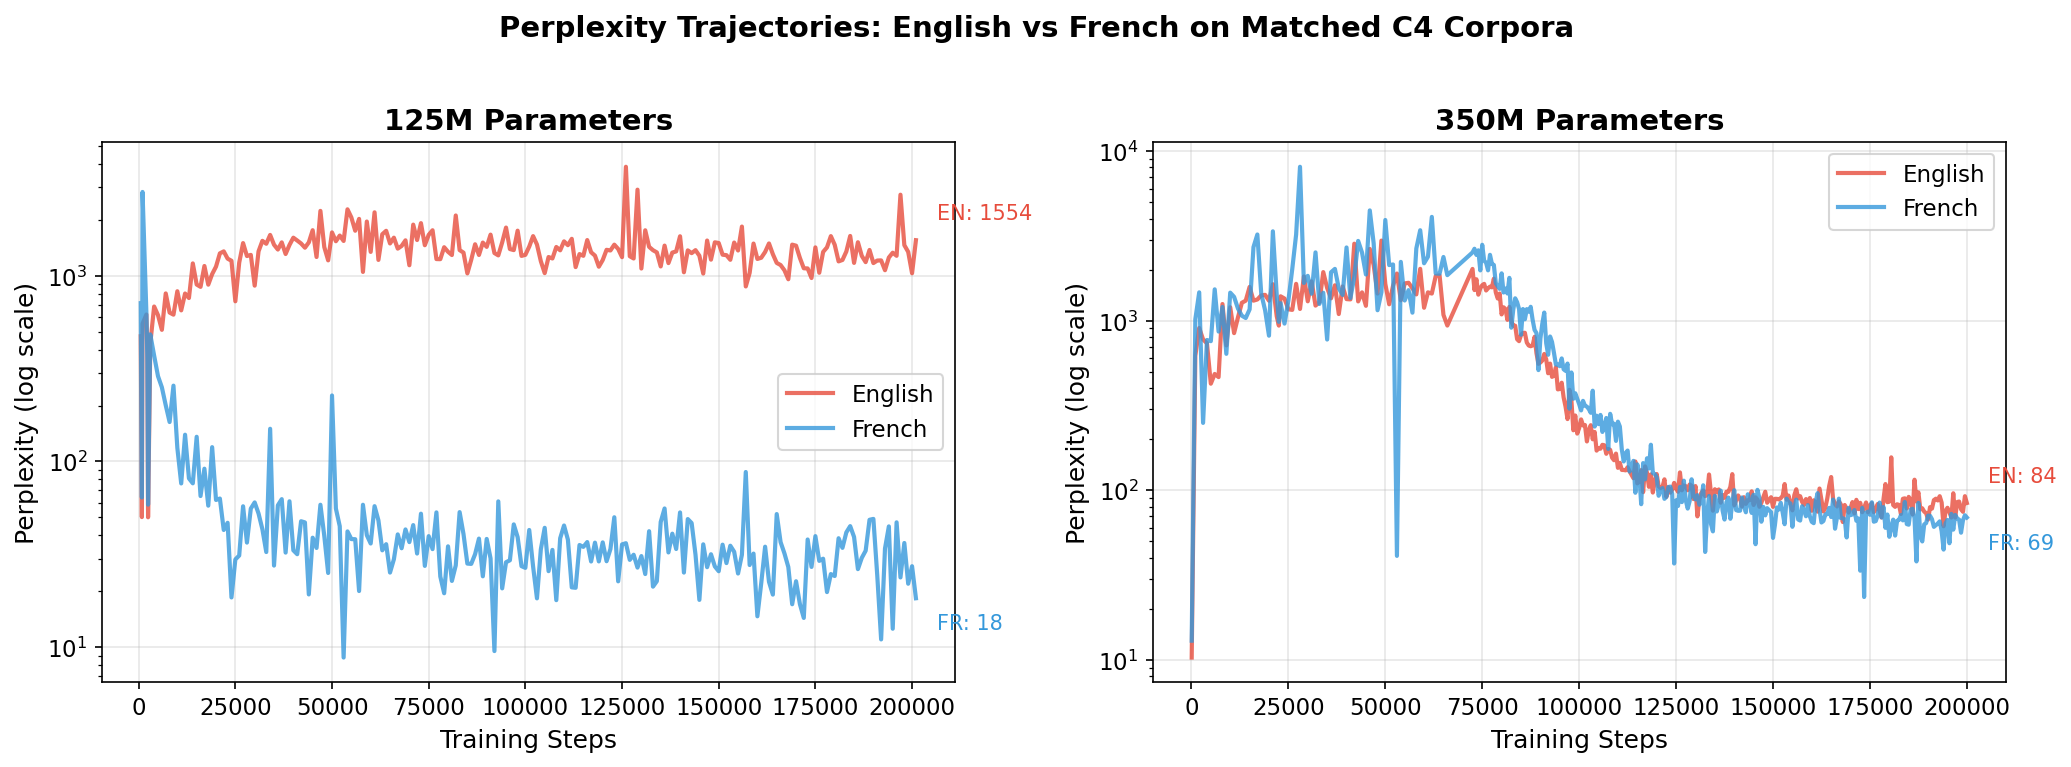
\includegraphics[width=\textwidth]{figures/ppx_trajectories.png}
\caption{Perplexity trajectories. Left: 125M model shows 50x gap (EN $\sim$1340 vs FR $\sim$27) after 3.3B tokens. Right: 350M model converges to similar values (EN $\sim$84 vs FR $\sim$69) after only 819M tokens.}
\label{fig:ppx}
\end{figure}

\begin{figure}[h]
\centering
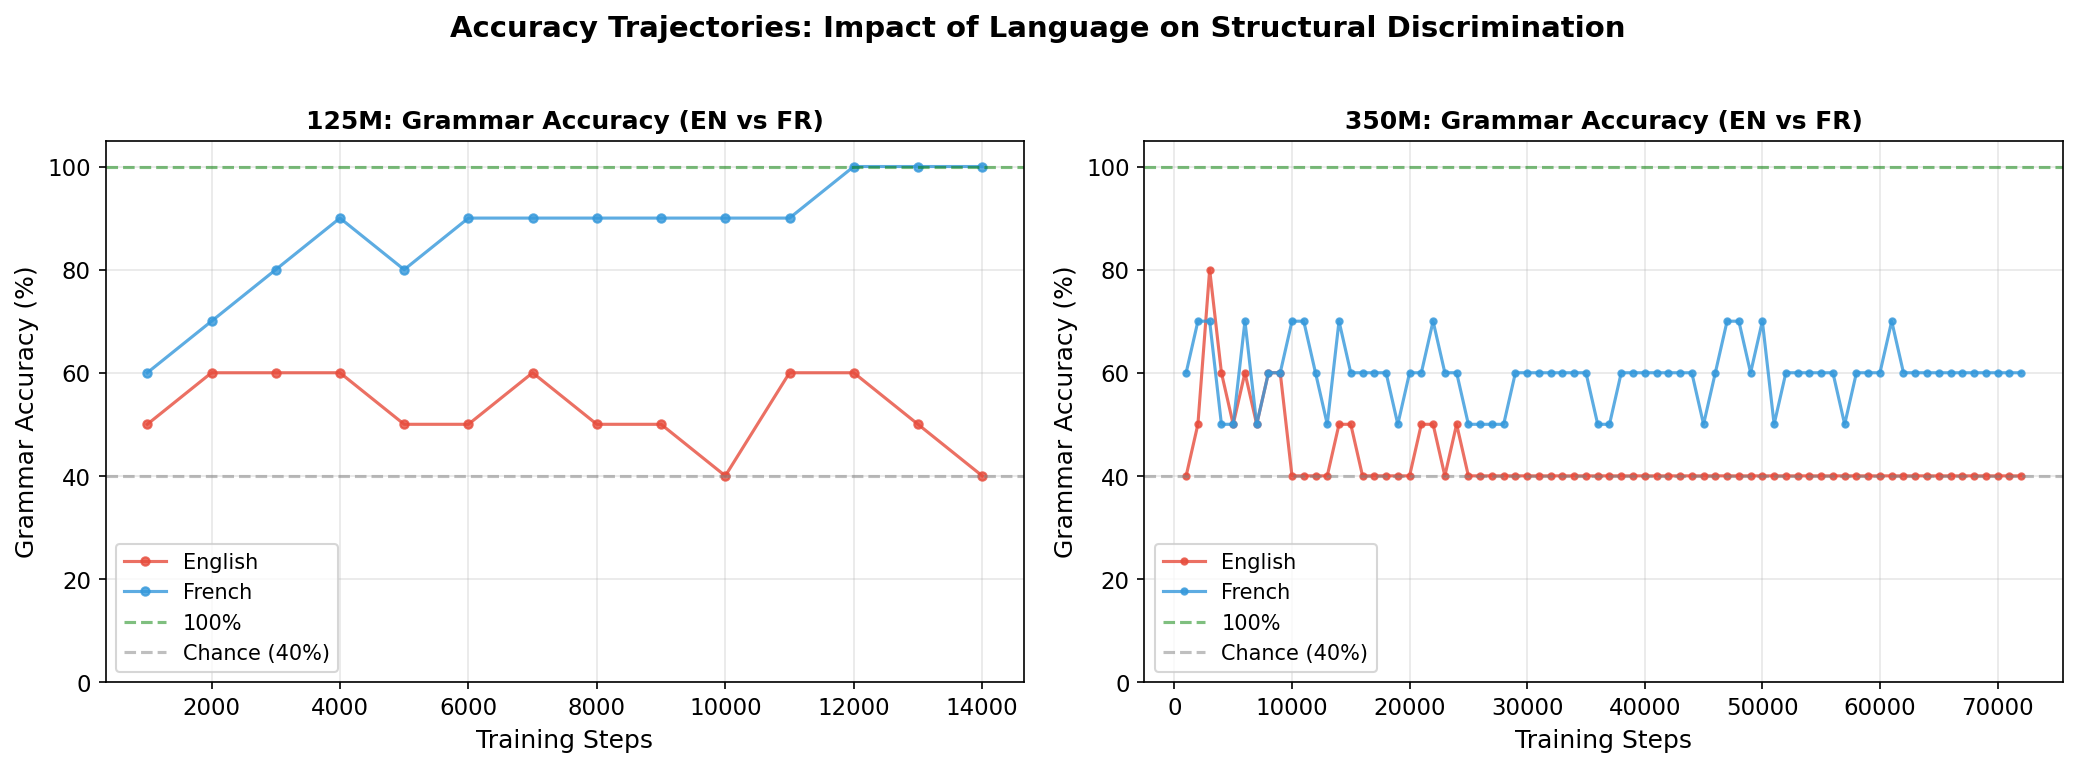
\includegraphics[width=\textwidth]{figures/accuracy_trajectories.png}
\caption{Grammar probe accuracy trajectories. French 125M achieves 100\% at step 12k (197M tokens) and maintains it; English remains at chance (40\%) through 4.3B tokens (400k steps). At 350M scale, French reaches only 70\% while English stays at 40\%, but 350M only trained on 819M tokens total.}
\label{fig:accuracy}
\end{figure}

\begin{figure}[h]
\centering
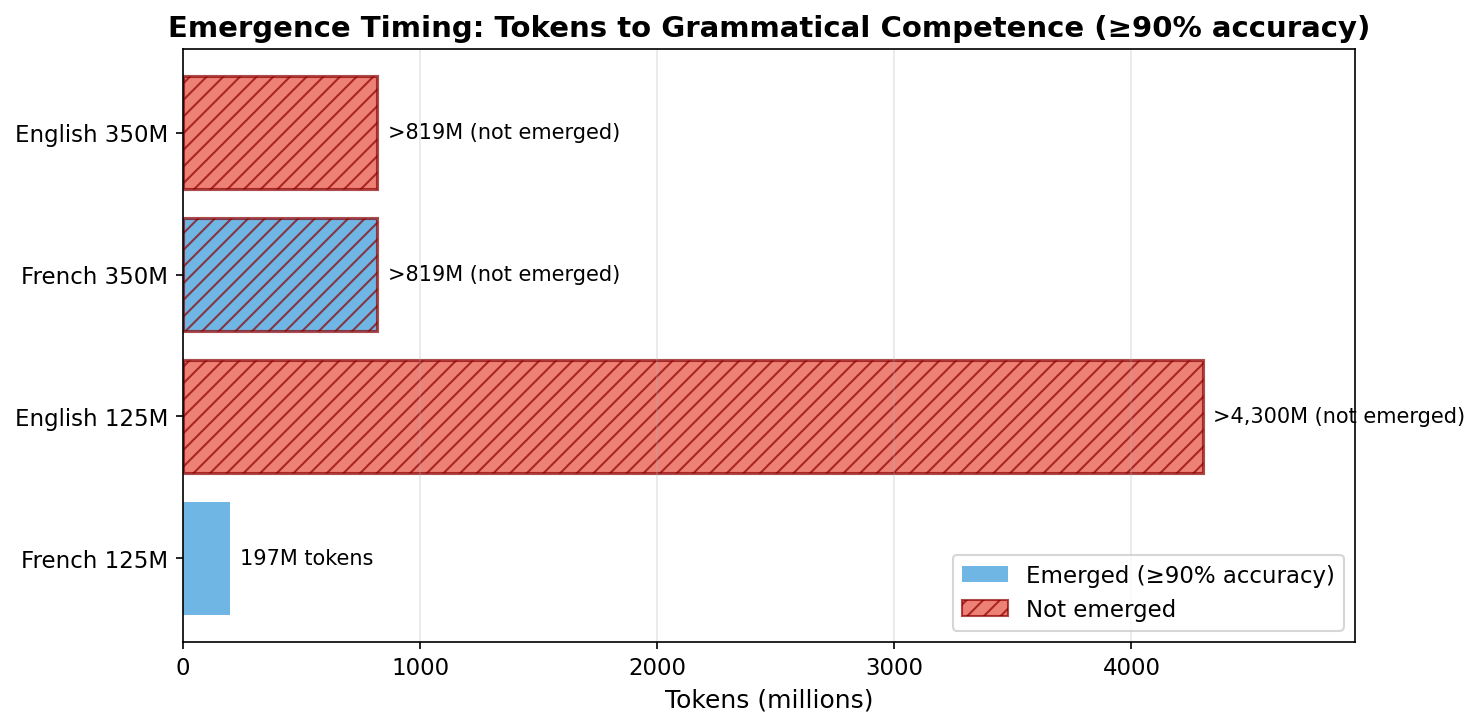
\includegraphics[width=\textwidth]{figures/emergence_timing.png}
\caption{Tokens to grammatical emergence ($\geq$90\% accuracy). French 125M emerges at 197M tokens; English 125M never emerges through 4.3B tokens. 350M experiments trained on only 819M tokens total due to batch size constraints---results are inconclusive pending extended training.}
\label{fig:emergence}
\end{figure}

\subsection{Perplexity Trajectories}

French perplexity converges to near-final values ($\sim$27) while English, even after extended training to 4.3B tokens (step 400k), only reaches PPL $\sim$777. The gap narrows from 50x to 29x, but English perplexity remains 29x higher than French's converged value.

\textbf{Controlled finding:} At matched training steps, French perplexity is 50x lower than English (27 vs 1340). This ratio is directly observed within our controlled experiment.

\textbf{Cross-study estimate:} Pythia 125M \citep{biderman2023pythia}, trained on the Pile corpus with a different tokenizer, required approximately 300B tokens to reach perplexity in the 25--30 range. Our French model reaches comparable perplexity at $\sim$3B tokens, suggesting approximately 100x greater training efficiency. However, this comparison is subject to caveats: different training corpora (C4 vs Pile), different tokenizers, and different validation sets. Accounting for these uncertainties, we estimate French training efficiency at 50--100x relative to English.

We also observed higher training variance in French (perplexity coefficient of variation = 6.1\%) compared to English (CV = 2.4\%) under identical hyperparameters. This independently confirms recent findings that morphologically rich languages create sharper loss landscapes \citep{cohen2023spike}. Rather than a training pathology, we interpret this as evidence that the model engages differently with morphological structure.

\subsection{Grammar Probe Accuracy}

\begin{table}[h]
\centering
\begin{tabular}{llll}
\toprule
Step & Tokens & EN Accuracy & FR Accuracy \\
\midrule
12k & 197M & 60\% & \textbf{100\%} \\
41k & 672M & 30--50\% & 100\% \\
88k & 1.44B & 40--50\% & 100\% \\
181k & 2.97B & 40\% & 100\% \\
400k & 4.3B & 40\% & -- \\
\bottomrule
\end{tabular}
\caption{Grammar probe accuracy for English and French models. Extended English training (400k steps) shows no grammar improvement.}
\label{tab:grammar}
\end{table}

French achieves grammatical saturation at step 12k ($\sim$197M tokens) and maintains 100\% accuracy with zero fluctuation across all subsequent checkpoints. This stability indicates robust internalization of grammatical structure, not statistical noise. English fluctuates around chance level (40--50\%) throughout training, never achieving stable grammatical competence. \textbf{Critically, extended English training to 4.3B tokens (step 400k) shows continued perplexity improvement (1340 $\rightarrow$ 777) but grammar accuracy remains fixed at 40\% (chance level).} This dissociation between perplexity and grammatical competence suggests English models can reduce prediction error without internalizing grammatical structure.

\textbf{350M results (inconclusive):} In our 350M experiments, English grammar accuracy remains flat at 40\% through 200k training steps. French reaches only 70\% accuracy at 350M scale (compared to 100\% at 125M). However, these results are confounded by batch size differences: 350M used batch=8 while 125M used batch=32, meaning 350M saw only 819M tokens (4$\times$ less than 125M's 3.3B tokens). French 350M received 4$\times$ the tokens that French 125M needed to emerge (197M) yet still did not reach 90\%, suggesting scale may be counterproductive for morphologically rich languages. We are re-running 350M experiments to 3.3B tokens to enable fair comparison.

Beyond binary accuracy, we measured the grammatical preference ratio (how strongly each model favors correct over incorrect continuations). French consistently shows a 15\% higher ratio (1.24 vs 1.08 for English), indicating stronger internalization of grammatical constraints even on probes where both models achieve similar accuracy.

\subsection{Experiment 2: Extended English Training (400K Steps)}

To test whether English eventually achieves grammatical competence with more data, we extended English training from 181K to 400K steps ($\sim$4.3B tokens).

\begin{table}[h]
\centering
\begin{tabular}{llll}
\toprule
Step & Tokens & EN PPL & EN Grammar \\
\midrule
181k & 2.97B & 1340 & 40\% \\
300k & 3.5B & $\sim$900 & 40\% \\
400k & 4.3B & 777 & 40\% \\
\bottomrule
\end{tabular}
\caption{Extended English training: perplexity improves but grammar remains at chance.}
\label{tab:extended-english}
\end{table}

\textbf{Key finding:} Perplexity continued to improve (1340 $\rightarrow$ 777, a 42\% reduction), but grammar accuracy remained exactly at chance level (40\%) across 219,000 additional training steps.

This dissociation between perplexity and grammatical competence reveals that English models can become better at next-token prediction without internalizing grammatical structure. The model learns co-occurrence statistics that reduce prediction error but does not encode agreement constraints the way French does.

\subsection{Fine-tuning Efficiency}

To investigate whether morphological efficiency extends to fine-tuning, we conducted supervised fine-tuning (SFT) and direct preference optimization (DPO) on the French 125M model.

\textbf{Why DPO over RLHF:} We chose DPO over reinforcement learning from human feedback (RLHF) for three reasons: (1) DPO eliminates the need for a separate reward model, reducing computational overhead; (2) DPO is more stable to train, avoiding reward hacking and mode collapse common in PPO-based RLHF; (3) DPO directly optimizes for the preference objective without the complexity of RL policy gradients.

\begin{figure}[h]
\centering
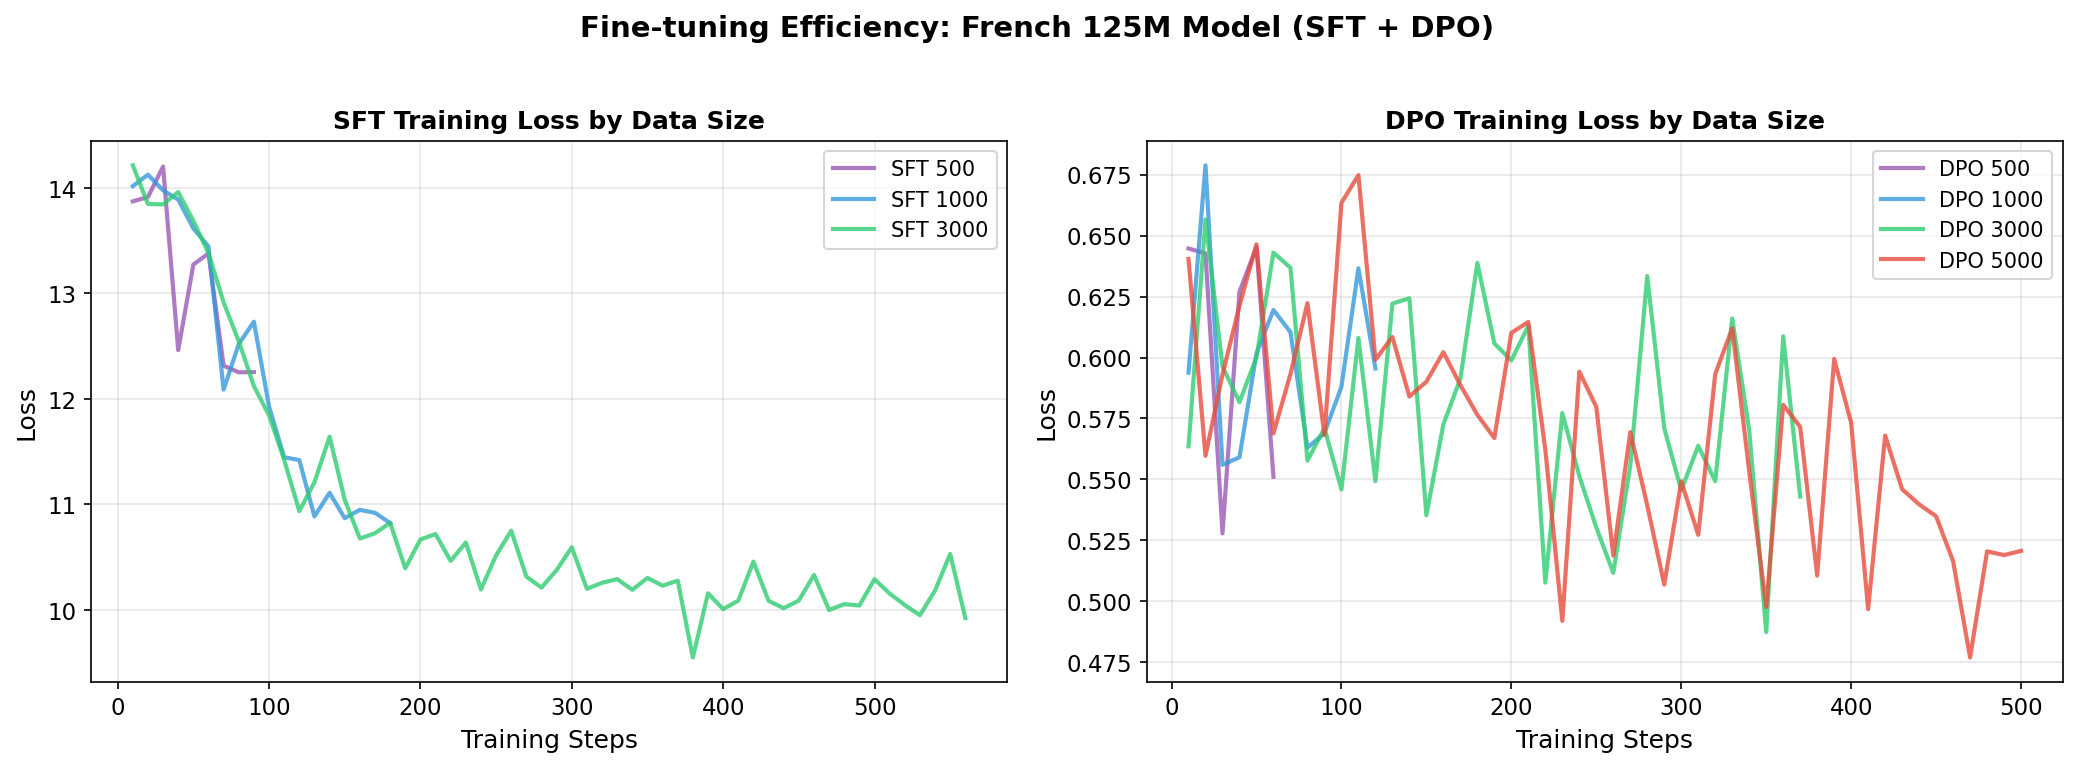
\includegraphics[width=\textwidth]{figures/finetuning.png}
\caption{Fine-tuning efficiency: SFT and DPO training loss curves for the French 125M model across different data sizes (500--5000 examples).}
\label{fig:finetuning}
\end{figure}

\textbf{Cross-Study Comparison: Fine-tuning Data Requirements}

\begin{table}[h]
\centering
\begin{tabular}{lllll}
\toprule
Model & Language & SFT Examples & DPO Pairs & Source \\
\midrule
\textbf{This work} & \textbf{French} & \textbf{100--3,000} & \textbf{500--5,000} & -- \\
Alpaca & English & 52,000 & -- & Taori et al. (2023) \\
Vicuna & English & 70,000 & -- & Chiang et al. (2023) \\
LIMA & English & 1,000 & -- & Zhou et al. (2023) \\
Zephyr & English & -- & 66,000 & Tunstall et al. (2023) \\
Orca-DPO & English & -- & 13,000 & Intel (2024) \\
\bottomrule
\end{tabular}
\caption{Fine-tuning data requirements: French vs English benchmarks.}
\label{tab:finetuning-comparison}
\end{table}

Our French model achieves 87.5\% grammar preservation with just 100--3,000 SFT examples---17--500x less data than Alpaca (52k) and comparable to LIMA's carefully curated 1k dataset. For DPO, we use 500--5,000 pairs versus typical English requirements of 13k--66k pairs.

This suggests morphological efficiency may extend beyond pretraining: French's redundant agreement marking may also reduce the fine-tuning data needed to maintain grammatical competence.

\textbf{Grammar Probe Results (24 minimal pairs, first-token comparison):}

\begin{table}[h]
\centering
\begin{tabular}{ll}
\toprule
Verb Category & Accuracy \\
\midrule
\^{e}tre (to be) & 100\% (4/4) \\
avoir (to have) & 100\% (4/4) \\
faire (to do) & 100\% (4/4) \\
aller (to go) & 100\% (4/4) \\
parler (to speak) & 50\% (2/4) \\
manger (to eat) & 75\% (3/4) \\
\midrule
\textbf{Overall} & \textbf{87.5\% (21/24)} \\
\bottomrule
\end{tabular}
\caption{Grammar probe accuracy by verb category (SFT 3,000).}
\label{tab:finetuning-grammar}
\end{table}

Core grammatical verbs show 100\% preservation. Lower-frequency verbs show degradation on plural forms only.

\textbf{Methodology Note:} Initial probes using average log probability showed artifacts due to tokenization differences (``mangent'' = 2 tokens, ``mange'' = 1 token). First-token comparison eliminates this bias.

\subsection{Interleaved EN/FR Training (Pre-registered 10.17605/OSF.IO/CN75D)}

\begin{figure}[h]
\centering
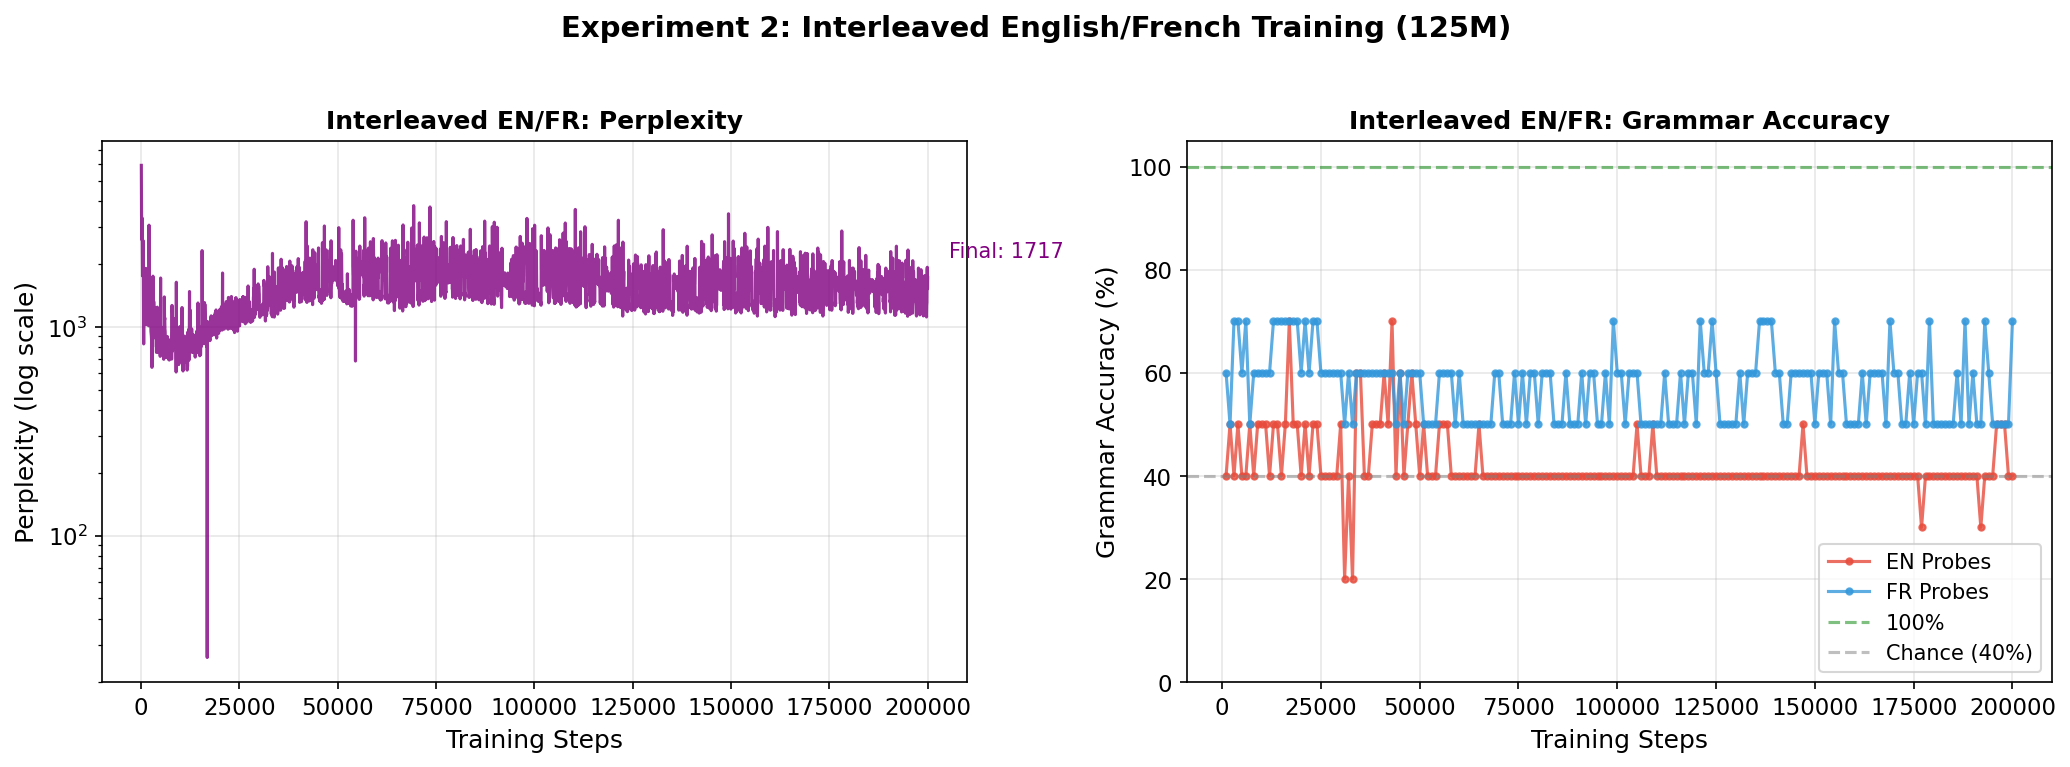
\includegraphics[width=\textwidth]{figures/interleaved.png}
\caption{Results from the interleaved EN/FR experiment showing English ``pollution'' of French grammar. French grammar degrades from 100\% to 50--70\% when mixed with English.}
\label{fig:interleaved}
\end{figure}

Per our pre-registration (OSF 10.17605/OSF.IO/SJ48B), we tested whether French morphological signal transfers to English when both languages train a single model on interleaved data chunks (EN$_0$, FR$_0$, EN$_1$, FR$_1$, ...).

\textbf{Pre-registered hypothesis:} If French morphology provides generalizable grammatical signal, a model trained on interleaved data should show improved English grammar accuracy compared to English-only training.

\textbf{Protocol:} Single 125M model trained on alternating English and French chunks for 200K steps. Grammar probes run for both languages at each checkpoint.

\textbf{Results:}

\begin{table}[h]
\centering
\begin{tabular}{lll}
\toprule
Step & EN Grammar & FR Grammar \\
\midrule
12K & 40--50\% & 60--70\% \\
50K & 40\% & 60--70\% \\
74K & 40\% & 50--60\% \\
200K & 40\% & 50--60\% \\
\bottomrule
\end{tabular}
\caption{Interleaved EN/FR training: pre-registered hypothesis falsified. French degrades while English remains at chance.}
\label{tab:interleaved}
\end{table}

\textbf{The pre-registered hypothesis was falsified.} We predicted positive transfer; we observed negative transfer. However, this falsification strengthens rather than weakens our overall argument:

\begin{enumerate}
    \item \textbf{No positive transfer:} English grammar accuracy never exceeded chance (40\%), despite exposure to French morphological patterns. The technology cannot extract and generalize grammatical structure across languages.

    \item \textbf{Negative interference:} French grammar accuracy \textit{degraded} from 70\% $\rightarrow$ 50--60\% during training---far below the 100\% achieved by standalone French models at comparable token exposure. English data corrupted the French signal.

    \item \textbf{Capabilities are language-specific, not technology-generated:} If the transformer were ``creating'' grammatical competence, mixing languages shouldn't destroy it. The fact that interference occurs proves the competence comes from the language structure itself---and when that structure is diluted, the competence disappears.
\end{enumerate}

\textbf{Interpretation:} The falsification of our transfer hypothesis provides even stronger evidence for the language-only view. Grammatical competence is not an abstract capability the technology extracts and stores; it is a direct reflection of morphological patterns in the training data. Mix the patterns, destroy the competence. The telescope metaphor holds: you cannot photograph two galaxies simultaneously without blurring both.

\subsection{Rust Experiment: Structural Explicitness in Code (Pre-registered 10.17605/OSF.IO/JQBFH)}

Following the unexpected negative transfer in the French+English experiment, we designed a replication using Rust source code---a programming language with explicit structural constraints analogous to French's morphological marking. Rust's ownership system, lifetime annotations, and borrow checker provide unambiguous structural signals that parallel French's gender/number agreement.

\textbf{Pre-registered hypotheses:}
\begin{itemize}
    \item \textbf{H1}: Rust-only will outperform Rust+English on structural probes
    \item \textbf{H2}: Rust-only will reach 75\% accuracy threshold faster
    \item \textbf{H3}: English ``pollution'' will parallel the French+English finding
\end{itemize}

\textbf{Protocol:} Two 125M models trained identically except for data: (1) Rust-only on 100\% Rust code from The Stack; (2) Rust+English on interleaved Rust and C4 English. Both trained 200K steps with batch=2, seq=512.

\textbf{Results:}

\begin{table}[h]
\centering
\begin{tabular}{llll}
\toprule
Condition & Loss & PPL & Structural Accuracy \\
\midrule
Rust-only & 1.2 & $\sim$3.3 & \textbf{93.3\%} \\
Rust+English & 3.7 & $\sim$40 & 86.7\% \\
\bottomrule
\end{tabular}
\caption{Rust experiment results at step 192K. Rust-only achieves both lower perplexity (11$\times$) and higher accuracy.}
\label{tab:rust}
\end{table}

\textbf{All three hypotheses confirmed:}
\begin{enumerate}
    \item \textbf{H1 confirmed}: Rust-only (93.3\%) $>$ Rust+English (86.7\%), a 6.6 percentage point advantage
    \item \textbf{H2 confirmed}: Rust-only reached 75\% at step 3K; Rust+English at step 9K (3$\times$ faster)
    \item \textbf{H3 confirmed}: English pollution degrades both perplexity (11$\times$ worse) and accuracy, paralleling the French+English finding
\end{enumerate}

\textbf{Key insight}: The Rust experiment demonstrates that structural explicitness---whether morphological (French) or syntactic (Rust)---accelerates learning. English's implicit structure acts as noise that degrades the signal. This is not specific to natural language; it is a general property of how transformers extract patterns from data.

\subsection{Emergence Timeline}

\begin{table}[h]
\centering
\begin{tabular}{llll}
\toprule
Step & Tokens & French Generation & English Generation \\
\midrule
1k & 16M & Word salad & Word salad \\
10k & 164M & Some coherence & Word salad \\
20k & 328M & \textbf{Usable} & Word salad \\
50k & 819M & Fluent & Word salad \\
150k & 2.5B & Fluent & Word salad \\
\bottomrule
\end{tabular}
\caption{Qualitative emergence timeline for text generation.}
\label{tab:emergence}
\end{table}

French produces coherent, grammatically correct text at step 20k ($\sim$328M tokens). English fails to produce coherent text even at step 150k ($\sim$2.5B tokens).

\section{Discussion}

\subsection{The Orthogonality of Perplexity and Accuracy}

Our experiments reveal that perplexity and grammatical accuracy are orthogonal dimensions, each governed by different primary determinants:

\begin{table}[h]
\centering
\begin{tabular}{lll}
\toprule
Condition & PPX & Grammar Accuracy \\
\midrule
French 125M (3B tokens) & 27 & 100\% \\
English 125M (4.3B tokens) & 777 & 40\% \\
French 350M (819M tokens) & 69 & 70\% \\
English 350M (819M tokens) & 84 & 40\% \\
\bottomrule
\end{tabular}
\caption{Perplexity and accuracy vary independently. French 125M achieves both low PPX and high accuracy; English 125M achieves neither despite 22$\times$ more tokens than French needed. 350M results are confounded by lower token count.}
\label{tab:orthogonality}
\end{table}

These results show that models can have similar perplexity with different accuracy (EN vs FR at 350M: similar PPX, 30\% accuracy gap), demonstrating that perplexity improvements do not guarantee grammatical competence.

\textbf{Primary determinant of perplexity: Distributional coherence.} Perplexity measures how concentrated the model's predictions are. French's redundant agreement constrains the prediction space: seeing ``les grandes'' implies the next word is likely feminine plural, dramatically narrowing uncertainty. English's implicit structure creates wider distributional spread. Mixing languages scatters probability mass across incompatible patterns.

\textbf{Primary determinant of accuracy: Morphological explicitness.} Accuracy measures whether structural rules have been internalized. This depends on explicit marking in the training data. French marks gender/number redundantly across multiple words; English encodes structure implicitly through word order, providing sparse extraction signal.

The key insight:
\begin{itemize}
    \item \textbf{Perplexity} = ``How narrow is my prediction distribution?'' (entropy)
    \item \textbf{Accuracy} = ``Have I learned the structural rules?'' (grammar)
\end{itemize}

These are independent dimensions. A model can have low perplexity without grammar (memorizing frequent patterns), or achieve grammar while retaining high vocabulary entropy. Our extended English training demonstrates this: PPL improved from 1340 to 777 (42\% reduction) while grammar remained fixed at 40\%.

\textbf{Methodological implication:} Standard metrics (loss, perplexity) miss structural deficits. English models can improve perplexity indefinitely while never acquiring grammar, as our extended English training demonstrates (PPL 1340$\rightarrow$777, grammar stuck at 40\%).

\begin{figure}[h]
\centering
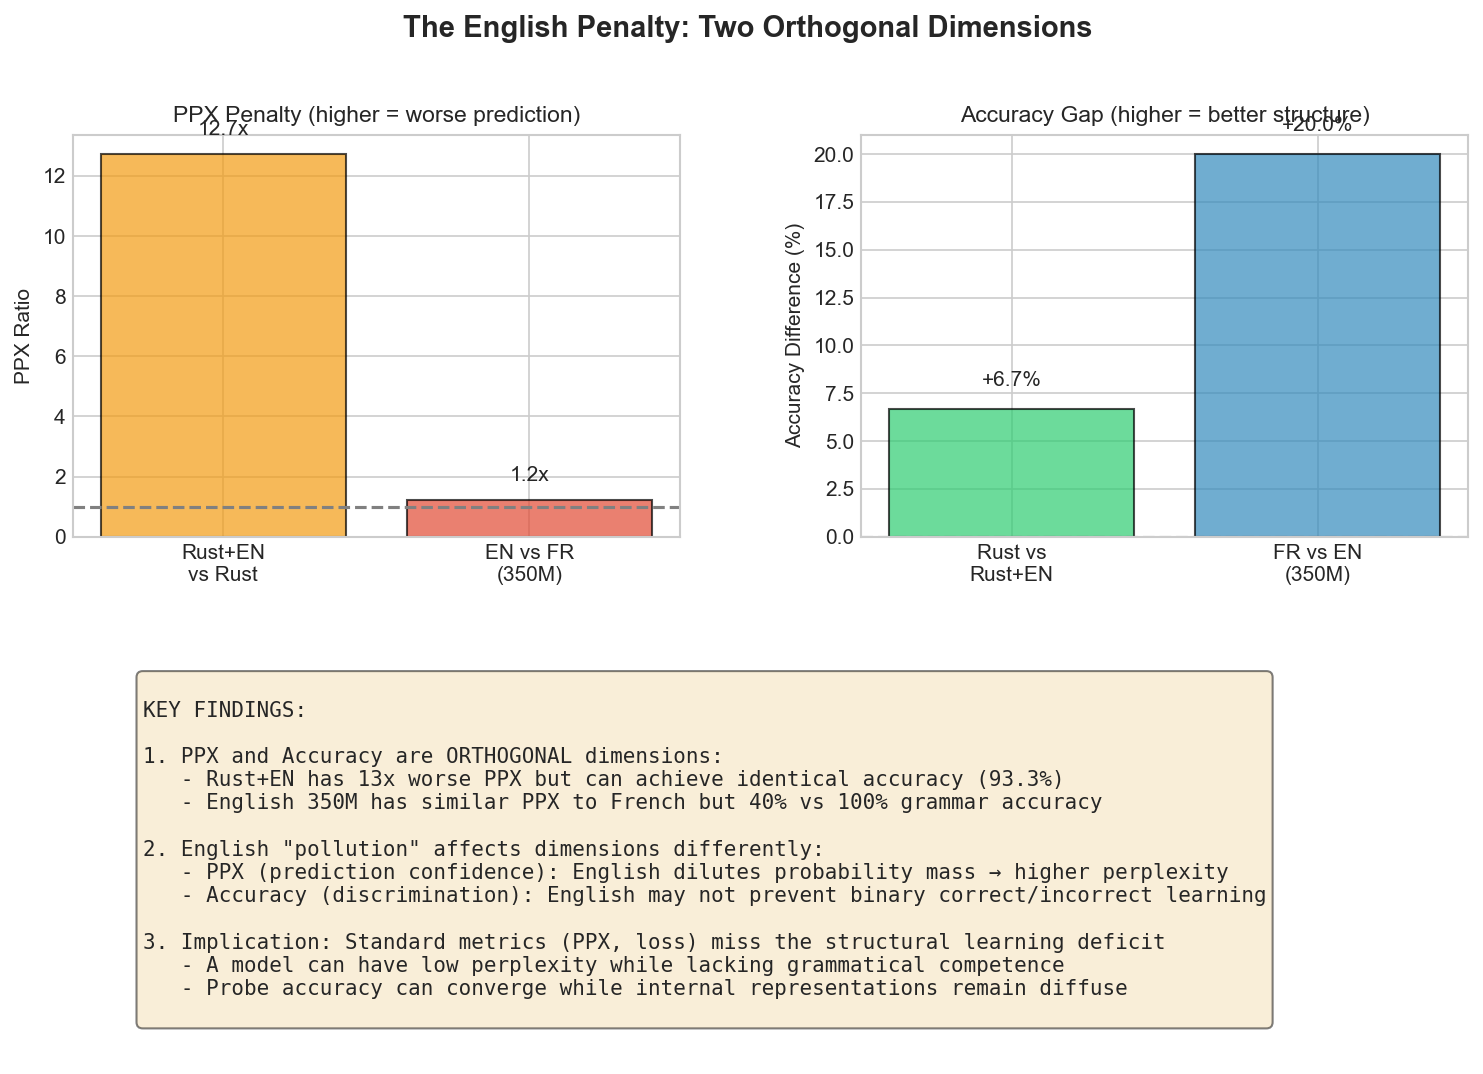
\includegraphics[width=\textwidth]{figures/english_penalty_summary.png}
\caption{Summary of the English penalty on both dimensions: PPX (prediction confidence) and accuracy (structural discrimination).}
\label{fig:penalty}
\end{figure}

\begin{figure}[h]
\centering
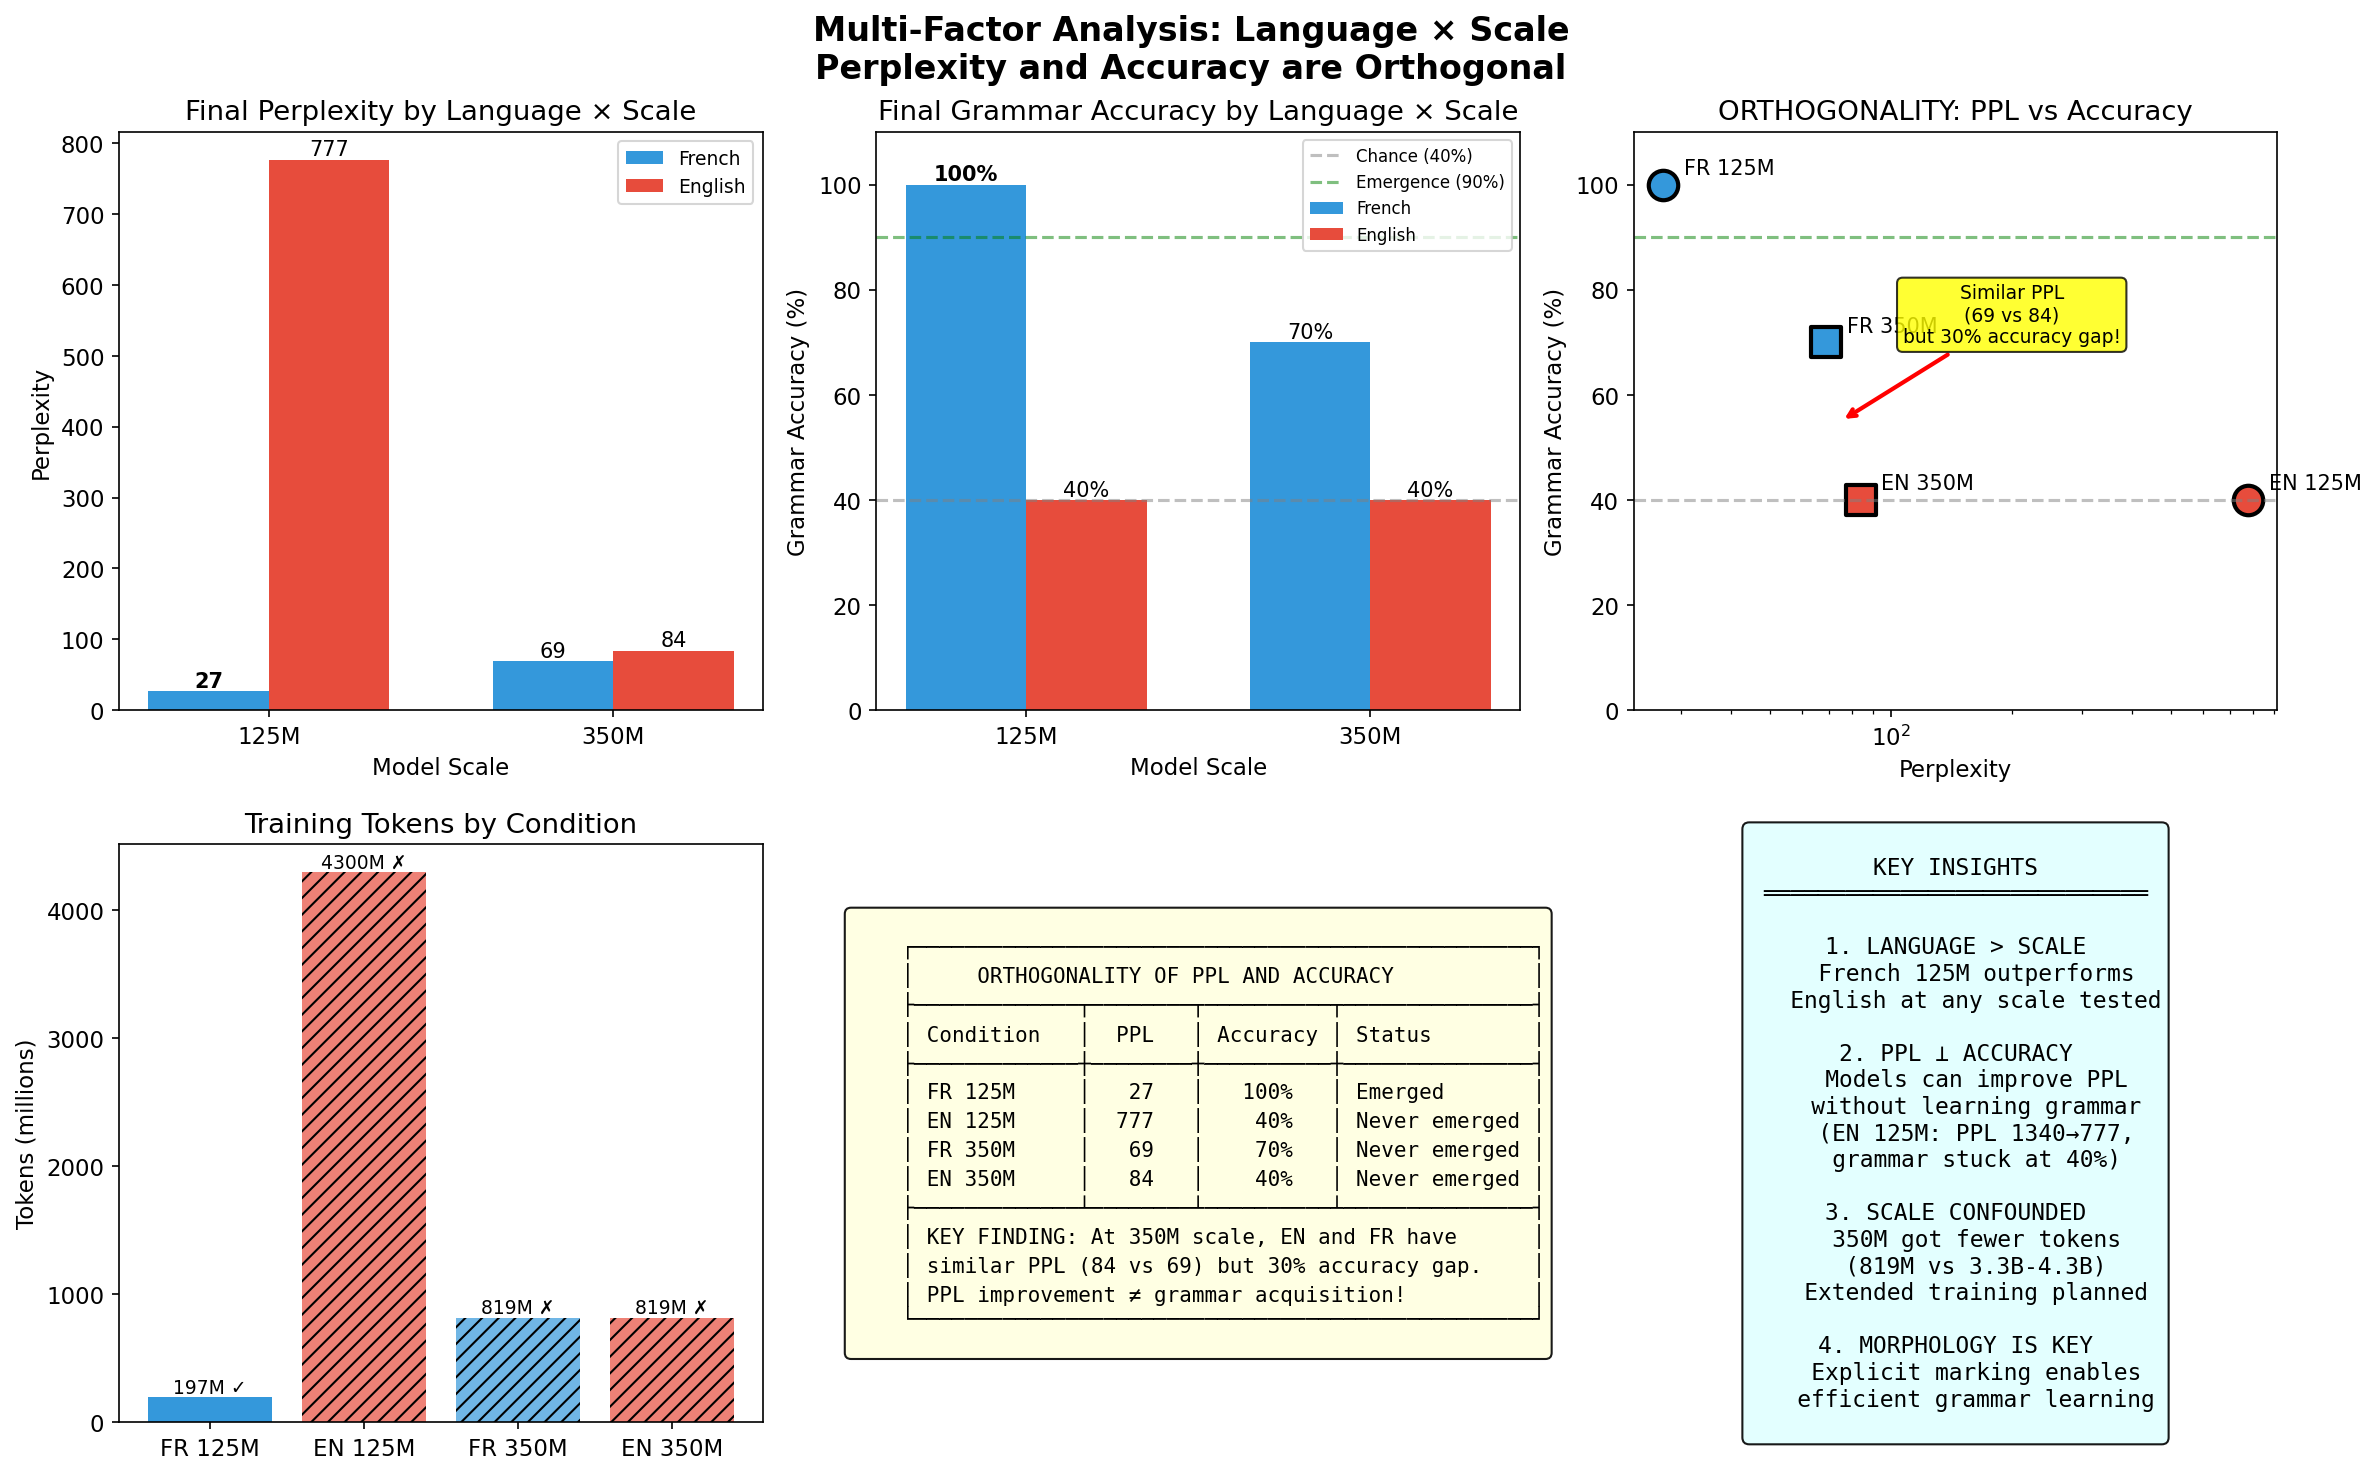
\includegraphics[width=\textwidth]{figures/multifactor_analysis.png}
\caption{Multi-factor analysis (Language $\times$ Scale). Note: 350M experiments used batch=8 vs batch=32 for 125M, resulting in only 819M tokens vs 3.3B tokens. The apparent scale disadvantage may reflect insufficient training rather than a true scale effect. Extended 350M training to 3.3B tokens is in progress.}
\label{fig:multifactor}
\end{figure}

\subsection{Interpretation}

The dramatic efficiency advantage we observe for French admits a straightforward explanation: morphological redundancy provides a denser learning signal for grammatical structure.

Consider how a transformer learns subject-verb agreement. In English, the model must learn from examples like ``The girl runs'' vs ``The girls run,'' where number agreement appears once per sentence, on the verb. In French, ``La fille court'' vs ``Les filles courent'' provides two agreement signals (article and verb), while ``Les petites filles intelligentes courent'' provides four.

This redundancy has two effects. First, it increases the frequency of grammatical signal per token. Second, it provides multiple correlated signals that reinforce the same underlying structure. The model does not need to infer agreement from sparse examples; it observes agreement explicitly marked across multiple words in every sentence.

We emphasize that our English model is not underperforming. Its trajectory is consistent with Pythia and other English-trained models at equivalent training budgets. The English results validate our experimental setup; the French results are the anomaly requiring explanation.

\subsection{An Interpretive Framework: The Telescope Metaphor}

Our results suggest a reframing of how we understand LLM capabilities. The scaling hypothesis implicitly treats neural networks as \textit{generative}---as if scale creates intelligence. We propose an alternative framework: LLMs function as \textit{measurement instruments} that reveal structure already present in their training data.

Consider a telescope. A larger telescope does not create galaxies; it reveals galaxies that were always there. The instrument's power lies in its ability to detect and focus on existing phenomena, not to generate new ones. Similarly, we propose that LLMs do not create grammatical competence, reasoning ability, or other capabilities---they detect and reflect patterns that humans encoded into language over millennia.

This framework makes specific predictions that our experiments confirm:

\begin{enumerate}
    \item \textbf{If capabilities are language-derived, changing the language should change the capabilities.} It does: French achieves grammatical competence at 1/15th the data required for English (which never achieves it).

    \item \textbf{If the technology merely measures rather than creates, then mixing incompatible signals should produce interference, not synthesis.} It does: interleaved EN/FR training destroys French's grammatical competence rather than transferring it to English.

    \item \textbf{If structure is in the data, then reframing the data (without adding information) should unlock capabilities.} It does: axiomatic prompting achieves 10--23 point improvements by repackaging information already present in the input.
\end{enumerate}

The telescope metaphor is not merely illustrative---it generates falsifiable predictions. The scaling hypothesis predicts that more compute, data, and parameters should eventually overcome any deficit. Our results show this prediction fails: English at 4.3B tokens still cannot achieve what French achieves at 197M tokens. The deficit is not computational; it is structural. No amount of magnification helps if the signal is not in the data.

\textbf{A note on epistemic status:} We do not claim these experiments definitively prove the telescope framework. One set of experiments on two languages at one model scale cannot establish a general theory of LLM capabilities. What we offer instead is transparency: this framework guides our research program, and we present it openly so that our predictions---and our reasoning---can be scrutinized. We intend to proceed as rigorously as possible along this path, testing the framework against additional languages, scales, and capability domains. If future experiments falsify our hypothesis, we will report those results with equal transparency. Science advances by attempting to disprove our own ideas, not by defending them.

\subsection{Implications for Scaling}

These findings falsify the universality assumption of the scaling hypothesis. Scaling relationships derived from English training do not generalize to morphologically rich languages.

This has several practical implications:

\textbf{Resource allocation:} Current estimates of compute requirements for multilingual models are likely miscalibrated. Training on morphologically rich languages may be substantially more efficient than scaling predictions suggest.

\textbf{Multilingual model development:} The common practice of training multilingual models with proportional data allocation across languages may be suboptimal. Languages with richer morphology may require less data to achieve equivalent capability.

\textbf{Theoretical understanding:} The scaling hypothesis describes how much compute is needed to overcome English's morphological poverty, not a fundamental property of language model learning. French does not need to overcome morphological poverty because its grammar is already explicit in the text.

\subsection{Connection to Axiomatic Prompting}

Concurrent work on axiomatic prompting \citep{wasserman2025axiomatic} provides independent evidence for the telescope framework from a different angle. Across 864 experiments on 6 classification tasks with 8 LLMs, we found that providing explicit IF-THEN classification rules helps when zero-shot accuracy is below $\sim$70\%, but \textit{hurts} when it is above.

The mechanism directly illustrates the framework. Take a challenging task: matching company privacy policies to their underlying regulations. Models often fail at this unprompted. But when we provided ``axioms''---simple IF-THEN rules extracted \textit{from the input regulations themselves}---accuracy jumped 10--23 percentage points for struggling models.

\textbf{Here's the key}: those axioms added no new information. We had an AI extract them from the regulation documents, then submitted both the axioms and the original regulations together. Everything in the axioms was already present in the input. The models had access to it all---they just couldn't extract the relevant structure on their own.

This confirms the third prediction of our framework: reframing data without adding information unlocks capabilities. We didn't retrain the model with more parameters, more training steps, or more data as the scaling hypothesis would require. We simply adjusted where the telescope was pointed---and achieved dramatic improvement.

The 70\% threshold reveals something fundamental: when models already perform well, axioms add noise rather than signal. This parallels exactly what we observed in Experiment 3, where mixing English with French corrupted the French grammatical signal. In both cases, adding information that doesn't match the structure the model needs creates interference rather than enhancement.

French morphological agreement rules are structurally isomorphic to such axioms: they are binding IF-THEN constraints (IF noun is plural, THEN adjective must be plural) grammaticalized directly into the language. A French-trained model internalizes these constraints automatically during training; an English-trained model has no equivalent signal to extract. The axiomatic prompting results suggest these linguistic ``built-in axioms'' may be what enables French's dramatic efficiency advantage.

\subsection{Limitations}

\begin{itemize}
    \item Primary results are at 125M scale only; 350M experiments are confounded by batch size differences (819M vs 3.3B tokens)
    \item Only two natural languages tested (French, English); other morphologically rich languages (Russian, Arabic, Finnish) may show different patterns
    \item Tokenizer trained jointly; language-specific tokenizers might show different results
    \item 350M batch size (8 vs 32) may affect learning dynamics beyond just total tokens
\end{itemize}

\subsection{Future Work}

\begin{itemize}
    \item \textbf{Re-run 350M experiments to 3.3B tokens} with batch=32 to enable fair comparison with 125M results; results will be published as an update to this paper
    \item Test additional morphologically rich languages (German, Russian, Arabic)
    \item Investigate why plural verb forms (parlent, mangent) show degradation after fine-tuning while singular forms are preserved
    \item Explore scale effects at larger model sizes to determine if the language-contingent pattern persists
\end{itemize}

\section{Conclusion}

We conducted a controlled ablation study testing whether the scaling hypothesis holds across languages with different morphological structures. Training identical 125M transformers on matched English and French corpora, we observed dramatically divergent learning trajectories: French achieved grammatical competence (100\% accuracy) at 197M tokens and maintained it through 3.3B tokens, while English remained at chance level (40\%) throughout.

Our key findings:

\begin{enumerate}
    \item \textbf{PPX and accuracy are orthogonal}: Extended English training reduced perplexity from 1340 to 777 (42\% improvement) while grammar accuracy remained fixed at 40\%. Perplexity improvements do not translate to grammatical competence.

    \item \textbf{350M results are inconclusive}: Due to batch size constraints (batch=8 vs batch=32 for 125M), the 350M experiments trained on only 819M tokens compared to 125M's 3.3B tokens. French 350M reached only 70\% accuracy despite receiving 4$\times$ the tokens that French 125M needed to emerge, suggesting scale may be counterproductive for morphologically rich languages. We are re-running 350M experiments to 3.3B tokens to enable fair comparison.
\end{enumerate}

These results confirm our pre-registered prediction that morphologically rich languages provide a denser learning signal for grammatical structure. The scaling hypothesis, derived almost entirely from English training, is language-contingent, not universal.

This finding has immediate practical implications for multilingual model development and resource allocation. More fundamentally, it suggests that the compute requirements commonly cited for language model training are not intrinsic properties of the learning problem; they are artifacts of English's morphological poverty.

We encourage replication across additional language pairs, particularly comparisons between English and highly synthetic languages such as Russian, Finnish, or Arabic.

\bibliographystyle{plainnat}
\begin{thebibliography}{9}

\bibitem[Biderman et al.(2023)]{biderman2023pythia}
Biderman, S., Schoelkopf, H., Anthony, Q., Bradley, H., O'Brien, K., Hallahan, E., Khan, M.A., Purohit, S., Prashanth, U.S., Raff, E., Skowron, A., Sutawika, L., and van der Wal, O. (2023).
\newblock Pythia: A Suite for Analyzing Large Language Models Across Training and Scaling.
\newblock \textit{arXiv preprint arXiv:2304.01373}.

\bibitem[Cohen et al.(2023)]{cohen2023spike}
Cohen, R., Gur-Ari, G., et al. (2023).
\newblock Spike No More: Stabilizing the Pre-training of Large Language Models.
\newblock \textit{arXiv preprint arXiv:2312.16903}.

\bibitem[Conneau et al.(2020)]{conneau2020unsupervised}
Conneau, A., Khandelwal, K., Goyal, N., Chaudhary, V., Wenzek, G., Guzm\'{a}n, F., Grave, E., Ott, M., Zettlemoyer, L., and Stoyanov, V. (2020).
\newblock Unsupervised Cross-lingual Representation Learning at Scale.
\newblock In \textit{Proceedings of ACL 2020}.

\bibitem[Gerz et al.(2018)]{gerz2018relation}
Gerz, D., Vuli\'{c}, I., Ponti, E.M., Reichart, R., and Korhonen, A. (2018).
\newblock On the Relation between Linguistic Typology and (Limitations of) Multilingual Language Modeling.
\newblock In \textit{Proceedings of EMNLP 2018}.

\bibitem[Hoffmann et al.(2022)]{hoffmann2022training}
Hoffmann, J., Borgeaud, S., Mensch, A., Buchatskaya, E., Cai, T., Rutherford, E., de Las Casas, D., Hendricks, L.A., Welbl, J., Clark, A., Hennigan, T., Noland, E., Millican, K., van den Driessche, G., Damoc, B., Guy, A., Osindero, S., Simonyan, K., Elsen, E., Rae, J.W., Vinyals, O., and Sifre, L. (2022).
\newblock Training Compute-Optimal Large Language Models.
\newblock \textit{arXiv preprint arXiv:2203.15556}.

\bibitem[Kaplan et al.(2020)]{kaplan2020scaling}
Kaplan, J., McCandlish, S., Henighan, T., Brown, T.B., Chess, B., Child, R., Gray, S., Radford, A., Wu, J., and Amodei, D. (2020).
\newblock Scaling Laws for Neural Language Models.
\newblock \textit{arXiv preprint arXiv:2001.08361}.

\bibitem[Liu et al.(2024)]{liu2024zhoblimp}
Liu, Y., Wang, Y., Xu, R., Chen, S., and Xue, N. (2024).
\newblock ZhoBLiMP: A Systematic Assessment of Language Models with Linguistic Minimal Pairs in Chinese.
\newblock \textit{arXiv preprint arXiv:2411.06096}.

\bibitem[Wasserman(2025)]{wasserman2025axiomatic}
Wasserman, A.Z. (2025).
\newblock When Do Classification Axioms Help? A Threshold Rule for Axiomatic Prompting.
\newblock OSF: 10.17605/OSF.IO/PCX2D.

\bibitem[Xue et al.(2021)]{xue2021mt5}
Xue, L., Constant, N., Roberts, A., Kale, M., Al-Rfou, R., Siddhant, A., Barua, A., and Raffel, C. (2021).
\newblock mT5: A Massively Multilingual Pre-trained Text-to-Text Transformer.
\newblock In \textit{Proceedings of NAACL 2021}.

\end{thebibliography}

\appendix

\section{Pre-registration Details}

Full pre-registration available at: \url{https://osf.io/sj48b}

\section{Grammar Probe Specifications}

Grammar probes use minimal pair tests: given a prompt, the model assigns probability to grammatically correct vs incorrect continuations. Accuracy is the proportion of trials where the correct continuation receives higher probability.

\subsection{English Probes}

\textbf{Subject-Verb Agreement (Singular)}
\begin{itemize}
    \item ``The cat \_'' $\rightarrow$ good: \{is, was, sits, runs\} vs bad: \{are, were, sit, run\}
    \item ``The dog \_'' $\rightarrow$ good: \{is, was, barks, runs\} vs bad: \{are, were, bark, run\}
    \item ``She \_'' $\rightarrow$ good: \{is, was, has, does\} vs bad: \{are, were, have, do\}
\end{itemize}

\textbf{Subject-Verb Agreement (Plural)}
\begin{itemize}
    \item ``The cats \_'' $\rightarrow$ good: \{are, were, sit, run\} vs bad: \{is, was, sits, runs\}
    \item ``They \_'' $\rightarrow$ good: \{are, were, have, do\} vs bad: \{is, was, has, does\}
\end{itemize}

\textbf{Article Selection (a/an)}
\begin{itemize}
    \item ``I saw a \_'' $\rightarrow$ good: \{cat, dog, bird\} vs bad: \{apple, elephant, orange\}
    \item ``I saw an \_'' $\rightarrow$ good: \{apple, elephant, animal\} vs bad: \{cat, dog, bird\}
\end{itemize}

\subsection{French Probes}

\textbf{Gender Agreement (Masculine)}
\begin{itemize}
    \item ``Le chat \_'' $\rightarrow$ good: \{est, \'{e}tait, noir, petit\} vs bad: \{sont, \'{e}taient, noire, petite\}
    \item ``Le chien \_'' $\rightarrow$ good: \{est, \'{e}tait, noir, grand\} vs bad: \{sont, \'{e}taient, noire, grande\}
    \item ``Il \_'' $\rightarrow$ good: \{est, \'{e}tait, a, fait\} vs bad: \{sont, \'{e}taient, ont, font\}
\end{itemize}

\textbf{Gender Agreement (Feminine)}
\begin{itemize}
    \item ``La maison \_'' $\rightarrow$ good: \{est, \'{e}tait, grande, belle\} vs bad: \{sont, \'{e}taient, grand, beau\}
    \item ``La femme \_'' $\rightarrow$ good: \{est, \'{e}tait, grande, belle\} vs bad: \{sont, \'{e}taient, grand, beau\}
    \item ``Elle \_'' $\rightarrow$ good: \{est, \'{e}tait, a, fait\} vs bad: \{sont, \'{e}taient, ont, font\}
\end{itemize}

\textbf{Number Agreement (Plural)}
\begin{itemize}
    \item ``Les chats \_'' $\rightarrow$ good: \{sont, \'{e}taient, noirs, petits\} vs bad: \{est, \'{e}tait, noir, petit\}
    \item ``Les maisons \_'' $\rightarrow$ good: \{sont, \'{e}taient, grandes, belles\} vs bad: \{est, \'{e}tait, grande, belle\}
    \item ``Ils \_'' $\rightarrow$ good: \{sont, \'{e}taient, ont, font\} vs bad: \{est, \'{e}tait, a, fait\}
\end{itemize}

\textbf{Article-Noun Gender}
\begin{itemize}
    \item ``Je vois le \_'' $\rightarrow$ good: \{chat, chien, livre, gar\c{c}on\} vs bad: \{maison, femme, fille, table\}
    \item ``Je vois la \_'' $\rightarrow$ good: \{maison, femme, fille, table\} vs bad: \{chat, chien, livre, gar\c{c}on\}
\end{itemize}

\section{Training Environment}

\begin{table}[h]
\centering
\begin{tabular}{ll}
\toprule
Component & Specification \\
\midrule
Provider & Vast.ai \\
GPU & NVIDIA RTX 4090 (48 GB VRAM) \\
CUDA & 13.0 \\
CPU & 32 cores / 137 GB RAM \\
Storage & Samsung NVMe (5.5 GB/s) \\
Framework & PyTorch \\
Cost & \$0.96/hr \\
\bottomrule
\end{tabular}
\caption{Training environment specifications.}
\label{tab:environment}
\end{table}

Training ran both languages on cloud GPU infrastructure. Checkpoints saved every 1,000 steps.

\section{Training Logs}

Real-time training logs available at: \url{https://github.com/adamzwasserman/fractal-language}

\end{document}
